\chapter{Learning Dynamics Appendix}
\section{Ressources}

\subsection{Data}
The GPT4 Alpaca dataset is collected from \url{https://huggingface.co/datasets/vicgalle/alpaca-gpt4}. 

\label{sec:alpaca-pres}
We define a taxonomy of 13 subtasks that the instructions can fall into: Classify, Code, Answer from Context (Question Answering based on a given passage), Create (Artistically oriented Natural Langiage Generation), Extract, Logic (Reasoning tasks), Answer from Memory (Question Answering from internal model knowledge), Summarize from Memory (Summarization/Explanation from internal model knowledge), Rewrite (Reformulation tasks), Write (Natural Language Generation tasks with a non-artistic goal), Summarize (Summarization tasks given a passage), Translate, and Other.
We then tag each of the 52000 instructions with the subtask it falls into using GPT4 as an oracle by prompting it with the classification task.
To verify the quality of the tagging, we manually verify a random sample of 100 instructions and find a 93\% agreement rate. 

The other datasets also originate from the HuggingFace Hub \footnote{\url{https://huggingface.co/datasets/glue}}\footnote{\url{https://huggingface.co/datasets/squad_v2}}\footnote{\url{https://huggingface.co/datasets/conll2003}}. We format all tasks as instructions using the following prompts and concatenating the input at the end.

\paragraph{MNLI} \sidecite{N18-1101} Classify the following relationship between the Hypothesis sentence and the Premise sentence, as either Entailment, Contradiction or Neutral. 

\paragraph{QNLI} \sidecite{wang2019glue, rajpurkar2016squad} Classify whether the given context contains enough information to answer the question (answerable) or not (unanswerable).

\paragraph{STSB} \sidecite{agirre-etal-2013-sem} Give an integer score between 1 and 5, describing how similar sentence1 and sentence2 are. 5 means they are very similar, 1 means they are nothing alike.

\paragraph{SST2} \sidecite{socher2013recursive} Classify the following sentence as negative or positive.

\paragraph{CONLL} \sidecite{tjong-kim-sang-de-meulder-2003-introduction} Extract locations, persons, and organizations from the text. The output should be formatted as a JSON object with three keys: LOC (locations), PER (persons), and ORG (organizations). Each key should have a value that is a list of strings. If the text contains no entities of a given type, the corresponding list should be empty.

\paragraph{SQUADV2} \sidecite{rajpurkar2016squad} Answer the question depending on the context. You must only answer with one excerpt from the text.

\paragraph{XSUM} \sidecite{Narayan2018DontGM} Summarize the following article in a few words.


Finally we split each data task category into 3 sets: a training set, a validation set, and a test set, with 80\%, 10\%, and 10\% of the data respectively.

\subsection{Models}
\label{sec:models}

Models are publicly available on the HuggingFace Hub, and are fairly similar decoder GPT architectures. We select the 7 billion parameter version to compare models with similar scales: \textbf{LLaMA} \sidecite{touvron2023llama},  \textbf{Falcon} \sidecite{penedo2023refinedweb}, \textbf{Pythia} \sidecite{biderman2023pythia}, \textbf{Bloom} \sidecite{scao2022bloom}).


\subsection{Metrics}
\label{sec:metrics}

Model performance is measured using two family of methods: \textit{reference-based metrics} and \textit{LM metrics}.

\paragraph{Reference-Based metrics} are the common metrics used in the litterature to evaluate the performance of a generative model on a given task, and offer a measure of the distance between a generation and a reference output. In this category are included the \textbf{Exact Match} and F-measures, but also more task-specific metrics based on co-occurence of words betwwen the output and the reference, such as \textbf{ROUGE} scores \sidecite{lin-2004-rouge} for summarization, BLEU scores for translation \sidecite{papineni-etal-2002-bleu}. To go beyond word matching heuristics, we also baseline neural network scorers. \textbf{SentenceBert} models \sidecite{reimers2019sentencebert} enables to calculate the cosine similarity between sentence embeddings; in this work a general purpose embedding model (all-mini-lm-l6-v2) is used. \textbf{BertScore} computes a F1 score leveraging pairwise cosine similarity between tokens, using a strong encoder model finetuned on an NLI task as shown to be best, here we use \texttt{microsoft/deberta-base-mnli} from the HuggingFace Hub \sidecite{he2023debertav3}.


\paragraph{LM metrics} are metrics that are computed by directly scoring the output using a language model. In this work, we experiment with \textbf{GPT4} and \textbf{GPT3.5} as scorers, by providing the evaluated model output and tasking the scorer to grade the quality of the output fom 0 to 10, based on relevance, fluency, factuality, coherence. The scoring prompts are task agnostic and allow to compare the performance of a model on different tasks, or on open-ended tasks where there is no ground truth and traditional literature metrics cannot be used. They also have the advantage of being continuous, which allows to study transitive regime without the "emergence" effect \sidecite{schaeffer2023emergent}. Finally, we baseline a \textbf{Reward Model (RM)} \sidecite{köpf2023openassistant}, a model trained on outputting a score designed to reflect a human's appreciation of a judgement. While this can be used as a reference-free scorer, we find increased robustness when reporting the score softmaxed with the RM score of the reference.

\paragraph{GPT Scoring prompt}
To obtain GPT4 and GPT3.5 scores for model responses to a given instruction, we prompt the OpenAI API as such:

\begin{quote}
You are a helpful assistant that helps evaluate the quality of two responses to a prompt.

Answer by awarding a score between 0 and 10 to each response, where 0 means the response is completely inappropriate and 10 means the response is very good.
A response that is acceptable should never be awarded less than 6 out of 10.

Answer base on the following criteria:\\
1. Is the response grammatically correct?\\
2. Is the response semantically correct?\\
3. Is the response coherent?\\
4. Is the response relevant to the prompt?\\

Output format (csv):\\
<score1 from 0 to 10>,<score2 from 0 to 10>\\

Rate the responses to the following instruction.\\
\{prompt\}

Response 1: 
\{response1\}


Response 2: 
\{response2\}

Output:
\end{quote}

Response 1 corresponds to the model prediction, and reference 2 to the "gold" label. The scores obtained are then checked for conformity (correct output template, scores between 0 and 10). Finally, they are scaled between 0 and 1.



\subsection{Framework}
Code is written using PyTorch and the Transformers library, as well as the PEFT library to train models using  low-rank adaptation. Training runs are done on compute clusters with NVIDIA V100 32GB GPUs.


\subsection{Default Model Training}
\label{sec:default-setup}
 We train models across a wide range of models, training data source and dataset sizes. To stay consistent between runs, we train models for 400 steps with a 128 batch size, achieved through gradient accumulation, a 5e-4 learning rate with linear decay, a warmup of 100 steps, or one epoch (whichever is lowest). We frequently log validation split CE loss and use early stopping to prevent overfitting. Code is fully released at \url{https://github.com/ManuelFay/IFTEval}. Training runs to completion take about 5 hours on a V100 GPU and 2h on a A100 GPU. This default setup is used to train all models in this work.

The only exception are models trained on datasets with less than 128 samples (less than the batch size). In these cases, we select a batch size of 8.


% \newpage
\section{Re-evaluating evaluation}


\subsection{Experimental setup}
\label{sec:exp_setup_1}

\textbf{Summarization dataset} In this dataset \sidecite{stiennon2022learning}, summaries are already generated and associated with human scores. We select 4 summarization models from the dataset, and 200 inputs the 4 models have been evaluated in common on, and that have at least 2 different human annotators. This enables computing Spearman Rank Correlation both between metrics and the mean human annotation, but also between human annotators by averaging the pairwise human correlation scores over all pairs of annotators.

\textbf{Synthetic Alpaca dataset}  Models are trained in the default conditions explicited in \ref{sec:default-setup}. To construct Spearman rank correlations between evaluators, we train a suite of over 52 models in which the training data mixture slightly differs (exclusion or partial exclusion of a target category). To do so, we (i) select one of the 13 task categories identified in \ref{sec:alpaca-pres}. (ii) We then build a base training data mixtures by concatenating the training splits from all other categories, respectively the validation splits. (iii) Finally, we randomly sample respectively 0, 10, 100 and 1000 samples from the held-out category's training split and add them to the base mixture. (v) We train one model per data mixture according to the training guidelines in \ref{sec:default-setup}. (v) We evaluate performance with all metrics on the held-out task test split. (vi) The process is repeated for all categories.


\textbf{Human-annotated datasets} Models are trained in the default conditions explicited in \ref{sec:default-setup}. To evaluate Spearman correlation between rankers (CAT and CIT scenarios), we train a suite of over 300 models in which the training data mixture slightly differs (exclusion or partial exclusion of a target category). To do so, we (i) select all 13 task categories identified in \ref{sec:alpaca-pres}. (ii) We then build a base training data mixtures by concatenating the training splits from all categories, respectively the validation splits. (iii) We then select a category from the benchmark tasks (MNLI, QNLI, STSB, SST2, Squad, XSum, CONLL). (iv) We randomly sample respectively 0, 10, 25, 50, 100, 200, 500 and 1000 samples from the selected category's training split and add them to the base mixture, and repeat the sampling process 4 times;, to obtain 7*8*4 = 504 data mixtures. (iv) We train one model per data mixture according to the training guidelines in \ref{sec:default-setup}. (v) We evaluate performance with GPT4 on the target task test split. (vi) To compute the Spearman correlations, we aim to reduce dataset specific formatting artefacts and thus only select models trained with less than 100 target task samples in the training mixture. Correlations are computed two ways, either by computing Spearman correlations per task category and averaging the correlation values with human judgement (CIT), or by computing correlations globally without considering task category information (CAT) enabling the study of cross-task scoring comparability. 

\textbf{TFA}
Finally, to compute the \texttt{TFA}, that is the relative performance improvements after format is learned, we select 3 target tasks, MNLI, QNLI, SST2. These datasets are the three datasets we have perfect sample-wise binary human evaluation for from the set of \emph{human data} benchmarks. From the suite of trained models, we select 5 base models finetuned on the Alpaca dataset, and for each task, 5 models trained on both Alpaca and 1000 samples of the target task. Previous experiments (\autoref{fig:exp1b_all}) have shown that on these datasets, format is generally learned after a few hundred samples. This enables us to compare models that learned target task output format with models that have not, using the various metrics at our disposal. We compute the relative performance improvement of all metrics, and average them in Tab. \ref{tab:main_metrics} (\texttt{TSA}). While human evaluation shows model performance has progressed with the introduction of target task samples (12\%), non-LLM metrics largely overestimate the boost in response performance, because of their strong bias towards outputs matching the "gold" reference. In low-shot settings when no formatting is learned, it is particularly interesting to use format agnostic scorers like GPT4 to truly analyze a model's comprehension of a task.

\subsection{Obtaining Human Scores on the benchmark data} 

To facilitate the collection of human annotated model outputs on the non-synthetic data, we simplify the problem by reducing it to a binary choice (Correct / Incorrect)  on classification-like datasets (SST2, MNLI, QNLI). We manually observe outputs for each trained model and output task category, and craft pre-tagging heuristics to make the annotation process quicker. These heuristics are empirically built with knowledge of model outputs; for example on zero-shot sentiment classification tasks, Llama models will often answer \emph{"The sentence is Positive"}, instead of \emph{"positive"}, but trivial heuristic functions can assist in tagging these as correct answers. This is facilitated by the fact output structure for a given model/task combination is often very similar (especially at low decoding temperatures), and we can iterate on these heuristic functions until no error is detected at all. For non-classification tasks, we adopt a strict rating scheme as well. NER responses through the CONLL 2003 task are considered correct only when the dictionary contains all correct key/value pairs with respect to the ground truth, but disregarding formatting artefacts. For SquadV2, an extractive task, we report the F1 intersection between the predicted answer span, and the correct answer, similarly as what is done in \sidecite{rajpurkar2016squad}. Finally, for summarization, we report ROUGE scores for XSUM as a reference point, but do not include these results with the other tasks during correlation computations, and rather compute human correlations using the human annotation dataset from \sidecite{stiennon2022learning}, for which we report results on Table  \ref{tab:main_metrics} (SUM).


Code is released at \url{https://github.com/ManuelFay/IFTEval}.

\subsection{Results on Alpaca test set}

The full results per category are reported in Table \ref{tab:exp1a}.

\begin{table*}
    \centering
    \begin{tabular}{lrrrrrrr}
        \toprule
         & GPT4 & GPT3.5 & ROUGE-1 & BERTScore & SBERT & RM & Soft RM \\
        \midrule
        Write & 0.97 & 0.86 & 0.41 & 0.72 & 0.74 & 3.21 & 0.33 \\
        Answer from Context & 0.94 & 0.86 & 0.55 & 0.76 & 0.80 & 1.29 & 0.45 \\
        Answer from Memory & 0.93 & 0.87 & 0.47 & 0.73 & 0.84 & 2.78 & 0.28 \\
        Extract & 0.92 & 0.88 & 0.54 & 0.77 & 0.83 & 1.61 & 0.52 \\
        Summarize from Memory & 0.92 & 0.85 & 0.45 & 0.73 & 0.84 & 3.21 & 0.43 \\
        Summarize from Context & 0.89 & 0.86 & 0.54 & 0.79 & 0.84 & 1.47 & 0.42 \\
        Rewrite & 0.89 & 0.87 & 0.68 & 0.86 & 0.82 & -0.20 & 0.47 \\
        Translate & 0.88 & 0.94 & 0.58 & 0.81 & 0.71 & 1.78 & 0.44 \\
        Create & 0.85 & 0.78 & 0.34 & 0.67 & 0.62 & -0.20 & 0.27 \\
        Classify & 0.85 & 0.76 & 0.50 & 0.73 & 0.72 & 0.74 & 0.43 \\
        Code & 0.79 & 0.82 & 0.46 & 0.71 & 0.74 & 0.73 & 0.43 \\
        Logic Reasoning & 0.71 & 0.88 & 0.52 & 0.73 & 0.80 & 0.33 & 0.49 \\
        \bottomrule
        \end{tabular}
    \caption[Averaged metric scores]{Averaged score over samples and models of each metric on each category. Category \textit{Other} is not listed as it  consists in synthetic instructions often not answerable by LLMs without external tooling.}
    \label{tab:exp1a}
\end{table*}


\subsection{Automatic Error Analysis}

To go further in the analysis and uncover novel insights at large scale, LLM models can for example enable automatic error analysis. We select a few low scoring outputs and prompt the scoring models to detect mistake patterns, or give potential explanations for the generative model's shortcomings On the sentiment classification task, automatic error analysis correctly detects that most errors are false positives, triggered by sarcasm, or "the presence of words that might be associated with positive sentiment in other contexts". For NLI tasks, it detects the tested model has troubles with  with "understanding negations, contradictions, and subtle differences in meaning between the premise and hypothesis".

\paragraph{Sentiment Analysis}
%Put in a figure
The following is a series of predictions a sentiment classification ML model got wrong. Can you spot any patterns in the types of mistakes the model made and explain in what areas the model needs to improve?

\begin{quote}
    

Sentence:
the château would have been benefited from a sharper , cleaner script before it went in front of the camera . 
Model prediction: The sentence is a positive statement.
Ground truth: negative

Sentence:
but there 's plenty to offend everyone ... 
Model prediction: The sentence is positive.
Ground truth: negative

Sentence:
outtakes in which most of the characters forget their lines and just utter ` uhhh , ' which is better than most of the writing in the movie 
Model prediction: The sentence is positive.
Ground truth: negative


Sentence:
the filmmakers ' paws , sad to say , 
Model prediction: The sentence is positive.
Ground truth: negative


Sentence:
in the media 
Model prediction: The sentence "in the media" is a positive statement.
Ground truth: negative


Sentence:
profanities 
Model prediction: The sentence "profanities" is a positive statement.
Ground truth: negative

\end{quote}

'The model seems to struggle with understanding the context and sarcasm in the sentences. It often misinterprets negative statements as positive, possibly due to the presence of words that might be associated with positive sentiment in other contexts. The model needs to improve in understanding the overall context of the sentences and detecting sarcasm or irony. Additionally, it seems to struggle with shorter sentences or single-word inputs, where it might not have enough information to accurately determine the sentiment.'


\paragraph{NLI}
The following is a series of predictions a NLI ML model got wrong. Can you spot any patterns in the types of mistakes the model made and explain in what areas the model needs to improve?


\begin{quote}
Premise:
He pulled his cloak tighter and wished for a moment that he had not shaved his head.
Hypothesis:
The man pulled his super hero cape around himself to show off.
Model prediction: Entailment.
Ground truth: neutral


Premise:
because i always had to do it and so i just pay someone else to do it and they do the they do the cutting they fertilize they um edge and um i think this year i'm going to have some landscaping put in
Hypothesis:
I still do all the gardening and landscaping myself. 
Model prediction: Entailment.
Ground truth: contradiction


Premise:
He's chosen Meg Ryan.
Hypothesis:
Jon Doe was chosen.
Model prediction: Entailment.
Ground truth: contradiction


Premise:
yep that's what he's worried about the trees or a bush because lilac bushes they they grow fast some people uh would really like to have them and then the people that do have them they spread and they sprout all over their their lawn
Hypothesis:
He's not worried about the trees. Lilac bushes take a long time to grow.
Model prediction: Entailment.
Ground truth: contradiction


Premise:
Trying Your Luck
Hypothesis:
This is not a game of luck, but one of pure skill.
Model prediction: Entailment.
Ground truth: contradiction


Premise:
He bent down to study the tiny little jeweled gears.
Hypothesis:
The were no jewels on the gears he examined.
Model prediction: Entailment.
Ground truth: contradiction


Premise:
As a basic guide, the symbols below have been used to indicate high-season rates in Hong Kong dollars, based on double occupancy, with bath or shower.
Hypothesis:
This page intentionally left blank.
Model prediction: Entailment.
Ground truth: contradiction


Premise:
In fact, European nations need to do some serious fiscal housecleaning.
Hypothesis:
There needs to be some serious fiscal housecleaning by European nations.
Model prediction: The relationship between the Premise sentence and the Hypothesis sentence is Neutral. The two sentences are not contradictory or entailing.
Ground truth: entailment


Premise:
It means that they gather and interpret their material fairly and argue about its interpretations rationally.
Hypothesis:
They gather and interpret the material fairly and argue rationally about it.
Model prediction: The relationship between the Premise sentence and the Hypothesis sentence is Neutral. Both sentences are independent of each other and do not entail or contradict each other.
Ground truth: entailment


Premise:
well that's pretty typical though uh i don't uh i don't guess it's going to be any much different uh than than it has been in the past so i expect uh July and August we'll see our  or uh share of hundred degree days
Hypothesis:
We don't ever see the temperature get into the hundreds.
Model prediction: Entailment.
Ground truth: contradiction


Premise:
They would burn to the ground by morning.
Hypothesis:
They would not burn to the ground by morning.
Model prediction: Entailment.
Ground truth: contradiction


Premise:
A rusty iron gate swinging dismally on its hinges! 
Hypothesis:
The iron gate did not move at all.  
Model prediction: Entailment.
Ground truth: contradiction


\end{quote}


The model seems to have a pattern of incorrectly predicting entailment when the ground truth is either neutral or contradiction. It appears to struggle with understanding negations, contradictions, and subtle differences in meaning between the premise and hypothesis. The model also seems to have difficulty with understanding the context and relationships between entities mentioned in the sentences.
To improve, the model needs to focus on better understanding negations, identifying contradictions, and recognizing subtle differences in meaning and context between sentences. Additionally, it should work on better identifying the relationships between entities and the overall context of the sentences.


\subsection{Correlations on the non-synthetic human tasks}

Table \ref{tab:exp1b_corr} and Table \ref{tab:exp1b_mean} display the scorer correlations between themselves on the non-synthetic datasets in both the \texttt{CAT} setting (Table \ref{tab:exp1b_corr}), and the \texttt{CIT} setting (Table \ref{tab:exp1b_mean}). Results are consistent with \autoref{fig:correlations}, with BertScore, SentenceBert, Rouge all displaying greater correlations between themselves than with reference-free metrics, and GPT4 standing out both on scoring within each tasks (CIT) and between tasks (CAT).


\begin{table*}
    \centering
    \begin{tabular}{lrrrrrrr}
    \toprule
     & ROUGE-1 & GPT4 & GPT3.5 & BScore & SBert & RM & Human \\
    \midrule
    ROUGE-1 & 1.00 & -0.16 & 0.46 & 0.73 & 0.85 & -0.77 & 0.22 \\
    GPT4 & -0.16 & 1.00 & -0.28 & 0.10 & -0.04 & 0.56 & 0.68 \\
    GPT3.5 & 0.46 & -0.28 & 1.00 & -0.00 & 0.16 & -0.37 & -0.19 \\
    BScore & 0.73 & 0.10 & -0.00 & 1.00 & 0.91 & -0.61 & 0.22 \\
    SBert & 0.85 & -0.04 & 0.16 & 0.91 & 1.00 & -0.69 & 0.29 \\
    RM & -0.77 & 0.56 & -0.37 & -0.61 & -0.69 & 1.00 & 0.28 \\
    Human & 0.22 & 0.68 & -0.19 & 0.22 & 0.29 & 0.28 & 1.00 \\
    \bottomrule
    \end{tabular}
    \caption[Spearman $\rho$ between scorers]{\textbf{Spearman $\rho$ between scorers} on non-synthetic data in the CAT setting.}
    \label{tab:exp1b_corr}
\end{table*}


\begin{table*}
    \centering
    \begin{tabular}{lrrrrrrr}
    \toprule
     & ROUGE-1 & GPT4 & GPT3.5 & BScore & SBert & RM & Human \\
    \midrule
    ROUGE-1 & 1.00 & 0.50 & 0.33 & 0.63 & 0.90 & -0.10 & 0.57 \\
    GPT4 & 0.50 & 1.00 & 0.66 & 0.07 & 0.35 & 0.40 & 0.77 \\
    GPT3.5 & 0.33 & 0.66 & 1.00 & -0.10 & 0.16 & 0.24 & 0.48 \\
    BScore & 0.63 & 0.07 & -0.10 & 1.00 & 0.66 & -0.43 & 0.13 \\
    SBert & 0.90 & 0.35 & 0.16 & 0.66 & 1.00 & -0.18 & 0.43 \\
    RM & -0.10 & 0.40 & 0.24 & -0.43 & -0.18 & 1.00 & 0.29 \\
    Human & 0.57 & 0.77 & 0.48 & 0.13 & 0.43 & 0.29 & 1.00 \\
    \bottomrule
    \end{tabular}
    \caption[Spearman $\rho$ between metrics]{\textbf{Spearman $\rho$ between metrics} on non-synthetic data in the CIT setting.}
    \label{tab:exp1b_mean}
\end{table*}

\section{IFT Models For Industrial Applications}

\subsection{$\mathcal{S}_1$: Improving Specific Tasks}

\subsubsection{Experimental setup}
\label{sec:exp_setup_app_31}
Models are trained in the default conditions explicited in \autoref{sec:default-setup}. To evaluate target task performance as target task samples are progressively introduced in the generalist synthetic training set, we train a suite, we (i) select all 13 task categories identified in \autoref{sec:alpaca-pres}. (ii) We then build a base training data mixtures by concatenating the training splits from all categories, respectively the validation splits. (iii) We then select a category from the benchmark tasks (MNLI, QNLI, STSB, SST2, SquadV2, Xsum, CONLL). (iv) We randomly sample respectively 0, 10, 25, 50, 100, 200, 500 and 1000 samples from the selected category's training split and add them to the base mixture, and repeat the sampling process 4 times;, to obtain 7*8*4 = 504 data mixtures. (iv) We train one model per data mixture according to the training guidelines in \autoref{sec:default-setup}. (v) We evaluate performance with all metrics listed in \autoref{sec:metrics} on the target task test split.

\begin{figure}[ht]
    \centering
    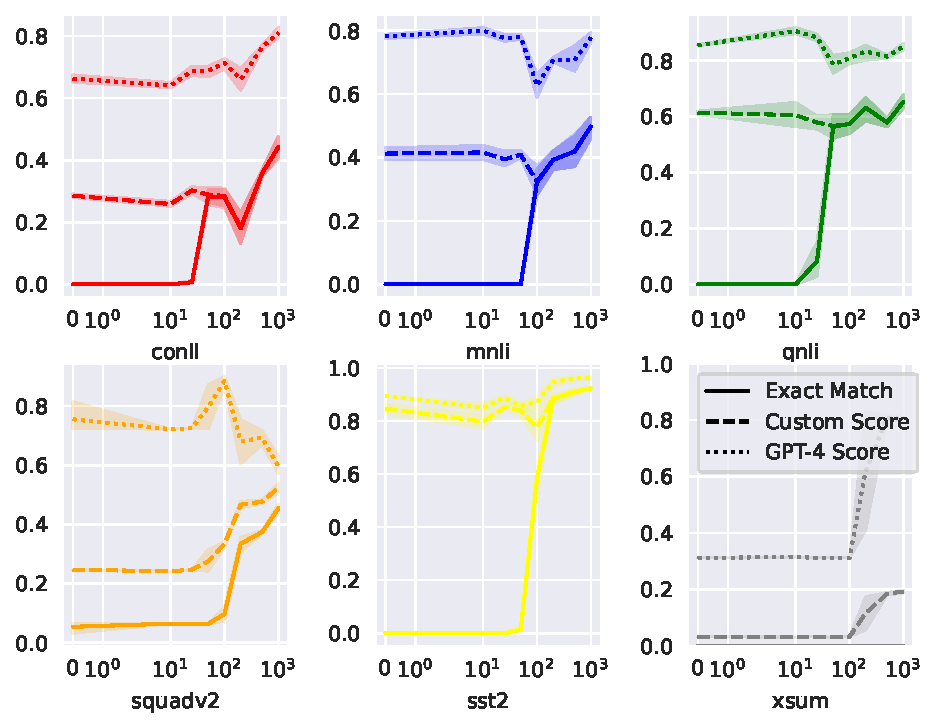
\includegraphics[width=0.5\textwidth]{images/learning_dynamics/exp1b_1.pdf}
    \caption[LLaMA performance with task samples]{LLaMA performance after incorporating $0 \leq N \leq 1000$ real task samples from respectively CONLL, MNLI, QNLI, SquadV2, SST2 and XSUM into the base training mixture}
    \label{fig:exp2}
\end{figure}


\subsubsection{Performance degradation}
\label{sec:app_perf_deg}
Full performance degradation results after 1000 samples of task-specific data are integrated within the synthetic test set are shown in \autoref{tab:perf_deg}.

\begin{table}
    \centering
    \begin{tabular}{lrrrrr}
    \toprule
     & Base & sst2 & conll & mnli & Average \\
    \midrule
    Bloom & 0.75 & 0.74 & 0.74 & 0.73 & 0.73 \\
    Falcon & 0.87 & 0.86 & 0.87 & 0.84 & 0.85 \\
    Llama & 0.84 & 0.85 & 0.86 & 0.86 & 0.86 \\
    Pythia & 0.67 & 0.66 & 0.66 & 0.66 & 0.66 \\
    \bottomrule
    \end{tabular}
    
    \caption[Alpaca test degradation]{Performance degradation on the Alpaca test set, after introducing 1000 samples of specialized data to the train set. Base denotes the reference scores, computed from the initial zero-shot performance.}
    \label{tab:perf_deg}
\end{table}



\subsection{$\mathcal{S}_2$: IFT models as Task-Specific Solvers}

\subsubsection{Experimental setup}
Models are trained in the default conditions explicited in \ref{sec:default-setup}. Starting from either a base model, or an instruction fine-tuned model, we evaluate target task performance as the model is fine-tuned solely on a varying number of target task training samples. We (i) select a target task from the real data benchmark tasks. (ii) We then sample a set of $N \in \{0, 10, 25, 50, 100, 200, 500, 1000\}$ samples from the training set, and pick 100 samples to serve as a validation split. (iii) We repeat the sampling process 4 times to mitigate variations between runs. (iv) We train one model per data mixture according to the training guidelines in \ref{sec:default-setup}. (v) We evaluate performance with all metrics listed in \ref{sec:metrics} on the target task test split.


\subsubsection{Extra models}
\label{sec:extra-datasets-exp4}
To evaluate the impact of IFT quality of the findings of the $\mathcal{S}_2$ experiment, we repeat the experiment using an "off-the-shelf" strong IFT model from the HuggingFace Hub. Notably, we select the 7B variant of \sidecite{vicuna2023} for the Llama variant, BloomZ for Bloom \sidecite{muennighoff2022crosslingual}, Falcon-Instruct for Falcon \sidecite{penedo2023refinedweb} and an IFT version of Pythia trained by \sidecite{köpf2023openassistant}. Results reported in Figure \ref{fig:exp4_old} show similar dynamics between the off-the-shelf models and the variants Instruction Fine-tuned in this work for one epoch on the Alpaca dataset \sidecite{alpaca2023}.

\begin{figure*}[ht]
    \centering
    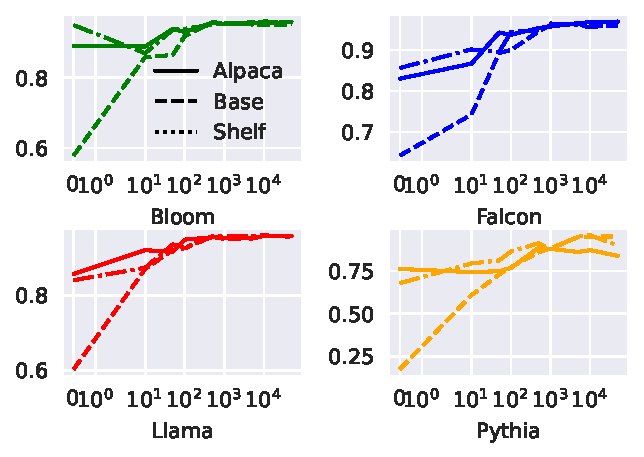
\includegraphics[width=0.8\textwidth]{images/learning_dynamics/exp4_all_old.pdf}
    \caption[GPT4 SST-2 scores]{GPT4 score on SST-2 test set after finetuning with $0 \leq N \leq 1000$  samples on a (base) LM, an "off-the-shelf" IFT model, and an IFT model fine-tuned on Alpaca.}
    \label{fig:exp4_old}
\end{figure*}
